% Created 2016-03-21 Mon 11:00
\documentclass[10pt,t,a4paper]{beamer}
\usepackage[utf8]{inputenc}
\usepackage[T1]{fontenc}
\usepackage{fixltx2e}
\usepackage{graphicx}
\usepackage{longtable}
\usepackage{float}
\usepackage{wrapfig}
\usepackage{rotating}
\usepackage[normalem]{ulem}
\usepackage{amsmath}
\usepackage{textcomp}
\usepackage{marvosym}
\usepackage{wasysym}
\usepackage{amssymb}
\usepackage{hyperref}
\tolerance=1000
\usetheme{BTH_msv}
\author{Mikael Svahnberg\thanks{Mikael.Svahnberg@bth.se}}
\date{2016-03-16}
\title{Use Cases \\\\ \texttt{PA14[13]5}}
\hypersetup{
  pdfkeywords={},
  pdfsubject={},
  pdfcreator={Emacs 25.1.50.1 (Org mode 8.2.10)}}
\begin{document}

\maketitle

\section{Use Cases}
\label{sec-1}
\begin{frame}[label=sec-1-1]{Use Case: Basic Notation}
\begin{itemize}
\item Narrative Document
\item Involves Actors and Events
\item Illustrates requirements in a story, in a timeline.
\item Considers the system as a \alert{black box}

\item Different levels:
\begin{itemize}
\item Brief (High Level)
\item Fully Dressed (Expanded)
\end{itemize}
\end{itemize}
\end{frame}
\begin{frame}[label=sec-1-2]{Example}
\begin{block}{Point Of Sale System}
A point of sale system (PoS, \href{http://www.urbandictionary.com/define.php?term=pos}{Don't look it up in UrbanDictionary}) is a computerised applicaion used to record sales and handle payments. It is typically used in a retail store. It includes hardware components such as a computer and a bar code scanner, and sofware to run the system.
\end{block}
\end{frame}
\begin{frame}[label=sec-1-3]{Functions in Example}
\begin{itemize}
\item Basic
\begin{itemize}
\item Record the current sale
\item Calculate current sales total
\item Reduce inventory after sale
\end{itemize}
\item Payment
\begin{itemize}
\item Handle Cash Payment
\item Handle Credit Payment
\item Log credit Payment
\end{itemize}
\item \ldots{}
\item \alert{Don't forget} quality attributes
\begin{itemize}
\item Response Time (Price will appear within 5 secs when recording a sold item)
\item Fault Tolerance (Must record payments to accounts within 24h)
\item System Requirements (Windows 10 or later)
\end{itemize}
\item Interface Requirements
\begin{itemize}
\item Methaphore (Shopping Basket)
\item Infrastructure (Platform: Windows 10, Database: MySQL, Programming Language: C++)
\end{itemize}
\end{itemize}

(Notice how we just ignored everything about requirements engineering best practices and went straight to the solution space)
\end{frame}

\begin{frame}[label=sec-1-4]{Example: Use Case}
\begin{verse}
Use Case: Buy Items \\
Actors: Customer, Cashier \\
Description: A customer arrives at a checkout with items to purchase. \\
\hspace*{3em}The cashier records the purchase item \\
\hspace*{6em}The system presents the running total and line-item details. \\
\hspace*{3em}The cashier collects the money and enters the payment information. \\
\hspace*{6em}The system updates inventory. \\
\hspace*{3em}The customer receives the receipt and leaves with the items \\
\end{verse}
\end{frame}
\begin{frame}[label=sec-1-5]{Actors}
\begin{itemize}
\item Actors are
\begin{itemize}
\item external to the system
\item participates in the story of a use case
\end{itemize}
\item System Boundary
\begin{itemize}
\item Hardware
\item Software
\item Organisation
\end{itemize}
\end{itemize}
\end{frame}
\begin{frame}[label=sec-1-6]{Use Case Diagrams}
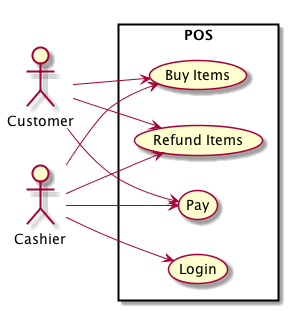
\includegraphics[height=6cm]{FUseCaseDiagram.png}
\end{frame}

\begin{frame}[label=sec-1-7]{Expanded Use Cases}
\begin{verse}
Use Case: <unique name of the use case> \\
Primary Actor: <Actor initiating the use case> \\
Stakeholders: <List of actors and their interests> \\
Purpose: <Intention of the use case> \\
\vspace*{1em}
Precondition: <What must be true before the use case can start> \\
Postcondition: <Guaranteed Results> \\
Overview: <High-level use case or other summary> \\
\vspace*{1em}
Basic Flow: <Main successful scenario> \\
Alternative Flows: <branches (success or failure) of the main scenario> \\
\vspace*{1em}
Special Requirements: \\
Technology: \\
Open Issues: \\
\end{verse}
\end{frame}
\begin{frame}[label=sec-1-8]{Expanded Use Case \\ Basic Flow}
Main Successful Scenario
\begin{center}
\begin{tabular}{p{5cm}p{5cm}}
Actor Action & System Response\\
\hline
1. The cashier records the purchase items & \\
 & 2. The system presents the running total and line-item details\\
3. The cashier collects the money and enters the payment information & \\
 & 4. The System updates the inventory\\
5. The customer receives the receipt and leaves with the items. & \\
\end{tabular}
\end{center}

Alternative Flows
\begin{verse}
Line n: \ldots{} \\
Line k: \ldots{} \\
\end{verse}
\end{frame}
\begin{frame}[shrink=20,label=sec-1-9]{Example of Expanded Use Case}
\begin{itemize}
\item Use Case:        Buy Items with Cash
\item Primary Actor:        Cashier
\item Stakeholders:        Customer, Company, Gvt., Tax agency
\item Purpose:                Capture a sale and its cash payment
\item Overview:
\end{itemize}
A customer arrives at a checkout with items to purchase.
The cashier records the purchase items and collects payment.
On completion, the customer leaves with the items.
\begin{itemize}
\item Precondition:        cashier is identified
\item Postcondition:        sale is safe, receipt is generated, payment is recorded
\item Basic Flow:
\begin{center}
\begin{tabular}{ll}
Actor Action & System Response\\
\hline
1. Customer arrives at a checkout with items to purchase. & \\
2. Cashier records identifier from each item. & \\
 & 3. The system determines the item price and adds item info into the sales transaction.\\
 & Description and price of the current item are presented.\\
 & \\
\end{tabular}
\end{center}
(Continues with more of the same)
\item Alternate Flows:
\begin{center}
\begin{tabular}{rl}
Line & Flow\\
\hline
2 & Invalid identifier is entered\\
 & The System indicates an error.\\
7 & Customer does not have enough cash\\
 & The Cashier cancels the transaction\\
\end{tabular}
\end{center}
\item Special Requirements:
\begin{itemize}
\item Touch Screen UI
\item Language Internationalisation
\end{itemize}
\item Technology:
\begin{itemize}
\item Item identifier entered by barcode laser scanner
\end{itemize}
\item Open Issues:
\begin{itemize}
\item Can the customer pay by card?
\end{itemize}
\end{itemize}
\end{frame}
\begin{frame}[label=sec-1-10]{Ranking Use Cases}
\begin{block}{Question}
Which use case is the most important to begin with?
\end{block}

\begin{block}{Rule}
First implement use cases that \emph{significantly influence} the core system architecture.

(Compare with Agile's \emph{Minimum Viable Product (MVP)})
\end{block}
\end{frame}
\begin{frame}[label=sec-1-11]{Ranking}
Increase ranking of a use case if it
\begin{itemize}
\item has direct impact on architectural design
\begin{itemize}
\item example: adds classes to domain layer, require persistent services
\end{itemize}
\item includes risky, time-critical, complex functions
\item involves new research or technology
\item represents primary business processes
\item directly supports revenue or decreased costs
\end{itemize}
\begin{block}{Ranking Techniques}
\begin{itemize}
\item Scored (Numerical Weights)
\item Discrete (High, Medium, Low)
\item Simple Ordering (bubble sort?)
\item MoSCoW (Must have, Should have, Could have, Won't have)
\item Cumulative Voting
\end{itemize}
\end{block}
\end{frame}
% Emacs 25.1.50.1 (Org mode 8.2.10)
\end{document}